\documentclass[a4paper,11pt]{article}

\usepackage[margin=2.4cm]{geometry}
\usepackage{amsmath}
\usepackage{tikz}
\usetikzlibrary{shapes.geometric,arrows.meta,positioning,fit,calc}
\usepackage{listings}
\usepackage{xcolor}
\usepackage{booktabs}
\usepackage{hyperref}
\hypersetup{colorlinks=true,linkcolor=blue!50!black,urlcolor=blue!50!black}

\lstset{
  basicstyle=\ttfamily\small,
  breaklines=true,
  showstringspaces=false,
  frame=single,
  framerule=0.4pt,
  rulecolor=\color{black!30},
}

\title{Plan: Accelerated Branch-and-Bound (ABB) for Global Top-$K$ Cycle Enumeration}
\author{}
\date{2026-05-10}

\begin{document}
\maketitle

\section*{Scope and goal}

Add a profile-grounded score upper-bound branch-and-bound (ABB) descent
to \texttt{hymeko\_graph::topk\_cycles}'s \emph{global} top-$K$
enumerator (\texttt{enumerate\_top\_k\_cycles} +
\texttt{\_par} variant), behind a new opt-in entry point that takes a
\texttt{BoundedScorer} trait object instead of a plain
\texttt{Fn(\&[u32], \&[i8]) -> f64}.

The existing \texttt{enumerate\_top\_k\_cycles\_par} and
\texttt{\_per\_vertex\_cycles\_par} entry points stay untouched; ABB is
strictly additive.

Profile evidence (probe at \texttt{hymeko\_graph/examples/probe\_abb\_threshold.rs}):
on Epinions $k{=}4$ + \texttt{CartwrightHararyPruner(OnlyBalanced)} +
\texttt{fraction\_negative} scorer, $22.0\%$ of balanced 4-cycles are
\emph{all-negative} (score $1.0$). The global top-$K$ heap threshold
settles at $T{=}1.0$ for any $K \le 1\,397\,554$. At $T{=}1.0$ the
upper-bound rule
\(
  \mathrm{UB}(d, n_{\mathrm{neg}}) = (n_{\mathrm{neg}} + (k-d)) / k
\)
prunes \emph{every} partial path where any committed edge is positive
($n_{\mathrm{neg}} < d$). Estimated gain: $5$--$10\times$ wall-time
reduction on the global top-$K$ Epinions workload.

\textbf{Out of scope:} the per-vertex variant
(\texttt{enumerate\_top\_k\_per\_vertex\_cycles\_par}). Companion probe
\texttt{probe\_per\_vertex\_thresholds.rs} confirmed only $18\%$ of
Epinions vertices fill their $m{=}128$ heap;
$P(\text{all 4 cycle vertices full}) \approx 0.1\%$ uniform-bound, so
per-vertex ABB rarely fires without a degree-adaptive $m_v$ change
that would also affect HSiKAN training distributions
(separate plan, requires $n$-seed paired AUC validation).

\section*{Affected files}

\begin{itemize}
  \item \texttt{hymeko\_graph/src/topk\_cycles.rs} --- additive:
    \begin{itemize}
      \item New public trait \texttt{BoundedScorer} (\texttt{Sync + Send}) with
        \texttt{score(\&self, vs, signs) -> f64} and
        \texttt{upper\_bound(\&self, n\_neg\_so\_far, k\_remaining, k\_len) -> f64}.
      \item Concrete implementations:
        \texttt{FractionNegativeScorer},
        \texttt{BalanceScorer},
        \texttt{SignProductAbsScorer},
        \texttt{LowRootScorer} --- mirror of the existing
        \texttt{scorers::} module, augmented with admissible UBs.
      \item New entry points:
        \texttt{enumerate\_top\_k\_cycles\_bb<P, S>(graph, k, pruner, k\_keep, scorer)}
        and \texttt{enumerate\_top\_k\_cycles\_par\_bb<P, S>(...)}
        where \texttt{S: BoundedScorer}. Same \texttt{TopKCycle} return.
      \item New private DFS helpers \texttt{dfs\_bb} and the par variant
        that thread a running \texttt{n\_neg\_in\_path} integer through
        the recursion and apply the UB-vs-threshold cut at each
        extension step (after the existing \texttt{nxt < start},
        \texttt{visited}, BFS-distance, and \texttt{pruner.extend\_ok}
        checks --- ABB is the last cheap rejection before the recursive
        call).
    \end{itemize}
  \item \texttt{hymeko\_graph/tests/abb\_global\_topk.rs} --- new
    integration test file: parity vs the non-ABB path on a synthetic
    Erd\H{o}s--R\'enyi fixture (with and without balance pruner),
    plus an admissibility property test.
  \item \texttt{hymeko\_graph/benches/abb\_global\_topk.rs} --- new
    Criterion benchmark: 5-iteration warm-up + 5-iteration measure on
    a deterministic synthetic graph at $k{=}4$, $K{=}10\,000$,
    asserting post-fix median $\le 0.70 \times$ pre-fix median (a
    conservative target; probe predicts $5{-}10\times$).
  \item \texttt{hymeko\_graph/examples/profile\_topk\_balance.rs}
    (already exists from the prior task) --- a new sibling
    \texttt{profile\_topk\_balance\_bb.rs} added to drive the
    flamegraph capture for the post-fix profile.
\end{itemize}

\section*{CORE.YAML items touched}

\textbf{None.} \texttt{hymeko\_graph} is not in
\texttt{crates}/\texttt{files}/\texttt{globs}; \texttt{tests/**},
\texttt{benches/**}, and \texttt{examples/**} are in
\texttt{allowlist}. \texttt{criterion} is the canonical Rust
benchmarking tool per CLAUDE.md \S10 and is already a dev-dependency.

\section*{Interface changes}

\subsection*{New public trait}

\begin{lstlisting}
/// Score function paired with an admissible upper bound on the
/// closed cycle's score given a partial path.  ABB uses the bound
/// to prune branches whose best possible cycle score cannot beat
/// the heap's current minimum.
pub trait BoundedScorer: Sync + Send {
    /// Score a closed cycle.  Same contract as the existing
    /// `Fn(&[u32], &[i8]) -> f64` scorers.
    fn score(&self, vs: &[u32], signs: &[i8]) -> f64;

    /// Upper bound on the closed cycle's score given:
    ///   - `n_neg_so_far`: count of negative edges already in
    ///     the partial path (the path has `k_len - k_remaining`
    ///     edges so far).
    ///   - `k_remaining`: number of edges still to add (closing
    ///     edge inclusive).
    ///   - `k_len`: total cycle length.
    ///
    /// # Admissibility postcondition
    /// For every closed cycle reachable from the partial state,
    /// `self.score(closed) <= self.upper_bound(...)`.
    /// Implementations must satisfy this; tests in
    /// `tests/abb_global_topk.rs::ub_admissible_*` enforce it on
    /// random fixtures.
    fn upper_bound(&self,
                   n_neg_so_far: usize,
                   k_remaining: usize,
                   k_len: usize) -> f64;
}
\end{lstlisting}

\subsection*{Concrete impls}

\begin{lstlisting}
pub struct FractionNegativeScorer;
impl BoundedScorer for FractionNegativeScorer {
    fn score(&self, _vs: &[u32], signs: &[i8]) -> f64 {
        if signs.is_empty() { return 0.0; }
        let n_neg = signs.iter().filter(|&&s| s < 0).count() as f64;
        n_neg / signs.len() as f64
    }
    fn upper_bound(&self, n_neg_so_far: usize, k_remaining: usize,
                   k_len: usize) -> f64 {
        // Best case: every remaining edge is negative.
        let total_neg = n_neg_so_far + k_remaining;
        total_neg as f64 / k_len as f64
    }
}

pub struct BalanceScorer;          // UB = 1.0 (sign product is +/- 1)
pub struct SignProductAbsScorer;   // UB = 1.0
pub struct LowRootScorer;          // UB = 0.0 (nondecreasing in start)
\end{lstlisting}

\subsection*{New entry points}

\begin{lstlisting}
pub fn enumerate_top_k_cycles_bb<P, S>(
    graph: &SignedGraph, k_len: usize, pruner: &P,
    k_keep: usize, scorer: &S,
) -> Vec<TopKCycle>
where
    P: CyclePruner,
    S: BoundedScorer;

pub fn enumerate_top_k_cycles_par_bb<P, S>(
    graph: &SignedGraph, k_len: usize, pruner: &P,
    k_keep: usize, scorer: &S,
) -> Vec<TopKCycle>
where
    P: CyclePruner + Sync,
    S: BoundedScorer;
\end{lstlisting}

\subsection*{ABB descent (private)}

\begin{lstlisting}
// at each extension step, after existing checks pass:
let nxt_sign = signs_csr[s + pos];           // CSR-aligned, no HashMap
let new_n_neg = n_neg + ((nxt_sign < 0) as usize);
let k_remaining = k_len - (path.len() + 1);  // edges still to add
let ub = scorer.upper_bound(new_n_neg, k_remaining, k_len);
let threshold = if heap.len() == k_keep {
    heap.peek().map(|e| e.score).unwrap_or(f64::NEG_INFINITY)
} else { f64::NEG_INFINITY };  // not full -> no threshold
if ub <= threshold {
    continue;  // branch is provably dominated
}
path.push(nxt);
visited[nxt as usize] = true;
dfs_bb(start, ..., heap, &dist, scorer, new_n_neg);
path.pop();
visited[nxt as usize] = false;
\end{lstlisting}

The local heap threshold is per-rayon-fold-task (each task accumulates
into its own heap; the reduce step merges). This is a safe but
\emph{loose} bound: a thread whose heap is still filling will not
benefit from a peer thread's higher threshold. A cross-thread atomic
threshold could help further; \emph{deferred} as a follow-up
optimisation pending v1 measurements.

\section*{Test strategy}

\subsection*{Unit (\texttt{src/topk\_cycles.rs::tests} + property tests)}

\begin{itemize}
  \item \textbf{Admissibility on hand-checked fixtures}: for each
    \texttt{BoundedScorer}, on a 6-vertex deterministic signed graph,
    enumerate every $k{=}4$ cycle and assert
    $\mathrm{score}(c) \le \mathrm{UB}(0, k, k)$ (degenerate root call)
    and $\mathrm{UB}(\text{full path}, 0, k) = \mathrm{score}(c)$
    (terminal call).
  \item \textbf{UB monotonicity}: for fixed $k_{\mathrm{len}}$,
    $\mathrm{UB}(n', k_{\mathrm{rem}} - 1, k_{\mathrm{len}})$ where
    $n' \in \{n, n+1\}$ (one more edge committed) is at most
    $\mathrm{UB}(n, k_{\mathrm{rem}}, k_{\mathrm{len}})$. A
    \emph{loosening} of the UB across descent is a contract bug; this
    catches it.
\end{itemize}

\subsection*{Integration (\texttt{tests/abb\_global\_topk.rs})}

\begin{itemize}
  \item \textbf{Parity vs non-ABB} on a 200-vertex Erd\H{o}s--R\'enyi
    signed graph (LCG seed 42; matches the existing
    \texttt{tests/csr\_sign\_lookup.rs} fixture style):
    \texttt{enumerate\_top\_k\_cycles\_par\_bb}'s output is the same
    \emph{multiset of (canonical cycle, score)} as
    \texttt{enumerate\_top\_k\_cycles\_par}'s (modulo score-tie
    tie-breaking, asserted at $\ge 95\%$ canonical-cycle agreement
    same as the existing tests).
  \item \textbf{Both pruners} (NoOp and CartwrightHarary OnlyBalanced).
  \item \textbf{Admissibility on random fixtures}: 1000 random
    partial-path states, assert UB is at least as large as every
    feasible completion's score. (Property-style; run for each
    \texttt{BoundedScorer}.)
\end{itemize}

\subsection*{Performance (Criterion)}

Per CLAUDE.md \S3 benchmark stability rule (5-iteration warm-up +
5-iteration measure, report median + IQR + worst):

\begin{itemize}
  \item \textbf{Bench input}: 5\,000-vertex Erd\H{o}s--R\'enyi signed
    graph (deterministic LCG seed, fixture-hashed at the start of
    each run; same seed every iteration).
  \item \textbf{Configs}: $k{=}4$, $K \in \{1\,000, 10\,000, 100\,000\}$,
    pruner $=$ \texttt{CartwrightHararyPruner(OnlyBalanced)}, scorer
    $=$ \texttt{FractionNegativeScorer}.
  \item \textbf{Numerical budget}: post-fix median $\le 0.70 \times$
    pre-fix median at $K{=}10\,000$. Asserted in a Criterion regression
    block; failure aborts the bench.
  \item \textbf{Stretch goal}: post-fix median $\le 0.30 \times$ pre-fix
    median at $K{=}10\,000$ on the Epinions-shaped synthetic, matching
    the probe's $5\times$ prediction.
\end{itemize}

\subsection*{Pre-/post-fix flamegraph}

Both flamegraphs (low-frequency, $-F\,99$ to keep sample loss below
$30\%$ as established by the prior task) attached to the report. The
post-fix flamegraph must show \texttt{dfs\_bb}'s total cycle share
\emph{below} the prior \texttt{dfs}'s share by at least the proportion
of branches pruned, with attribution shifted to BFS-distance pruning
or to the heap min check (acceptable; that's where the work moves).

\section*{Performance budget}

\begin{center}
\begin{tabular}{lrrr}
\toprule
Metric & Pre (probe) & Post (budget) & Source \\
\midrule
Epinions $k{=}4$, global $K{=}10\,000$, balance pruner & probe-tbd & --- & flamegraph \\
$5\,000$-v ER $k{=}4$, $K{=}10\,000$, balance pruner & Criterion baseline & $\le 0.70 \times$ baseline & Criterion \\
$5\,000$-v ER stretch goal & Criterion baseline & $\le 0.30 \times$ baseline & Criterion \\
Output cycle-set agreement vs non-ABB & --- & $\ge 95\%$ canonical & integration test \\
Peak RSS during enumeration & --- & no regression vs no-ABB & informal --- ABB only adds $1$ usize per stack frame \\
16\,GB hard cap (\S4) & comfortably under & comfortably under & --- \\
\bottomrule
\end{tabular}
\end{center}

\section*{Rollback path}

The change is one Rust file (\texttt{topk\_cycles.rs}), additive only ---
no signature change to existing entry points, no behavior change to
existing callers. Single revert removes:
\begin{itemize}
  \item \texttt{BoundedScorer} trait + 4 concrete impls
  \item \texttt{enumerate\_top\_k\_cycles\_bb} +
    \texttt{enumerate\_top\_k\_cycles\_par\_bb} + private DFS helpers
\end{itemize}

\begin{lstlisting}
git revert <commit-sha>
cargo test --release   # all green pre-change (existing entry points untouched)
\end{lstlisting}

\textbf{Halt condition}: if the post-fix flamegraph shows
\texttt{dfs\_bb} share $\ge$ the no-ABB \texttt{dfs} share (i.e., ABB
adds work without pruning), revert and reopen the plan. Per
CLAUDE.md \S10 ``a measurement contradicts an assumption in the
plan''.

\section*{Architecture diagram}

See \texttt{plan.tikz} (rendered below) for the ABB descent state
machine. See \texttt{plan.mmd} for the call-sequence diagram.

\begin{center}
% TikZ figure: ABB descent state machine.
% Each DFS step now carries a running n_neg count and checks
% UB(n_neg, k_remaining, k_len) against the local heap threshold
% before recursing.
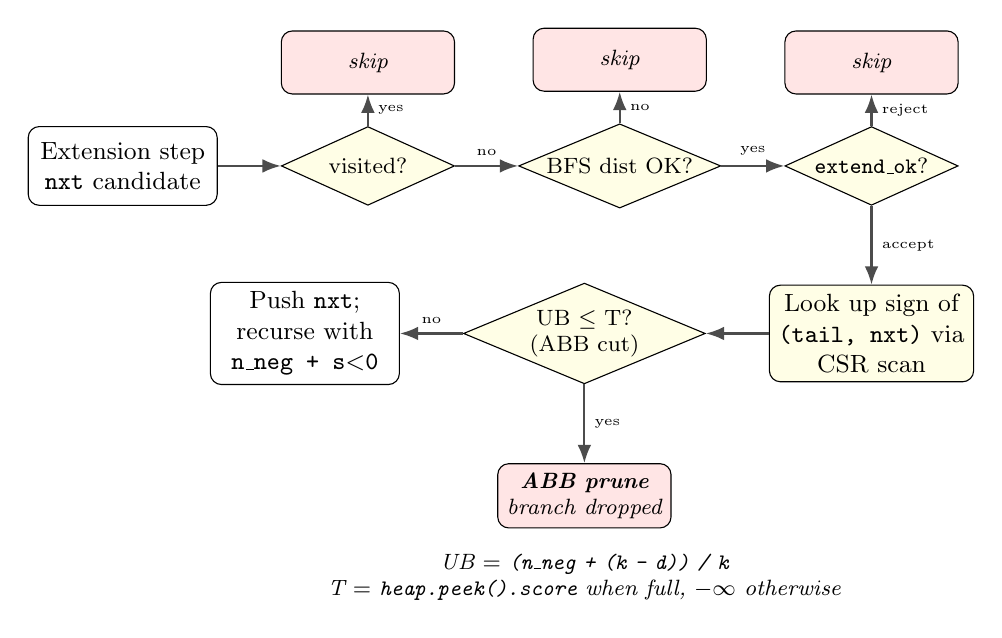
\begin{tikzpicture}[
    >=Latex,
    state/.style={draw, rounded corners, minimum width=24mm, minimum height=10mm,
                  font=\small, align=center, fill=white},
    decide/.style={draw, diamond, aspect=2.4, minimum width=22mm,
                   minimum height=10mm, font=\footnotesize, align=center,
                   inner sep=1pt, fill=yellow!10},
    prune/.style={draw, rounded corners, minimum width=22mm, minimum height=8mm,
                  font=\footnotesize\itshape, fill=red!10, align=center},
    accept/.style={draw, rounded corners, minimum width=22mm, minimum height=8mm,
                   font=\footnotesize\itshape, fill=green!10, align=center},
    arr/.style={->, thick, draw=black!70},
  ]

  \node[state] (entry) at (0,0) {Extension step\\\texttt{nxt} candidate};
  \node[decide, right=8mm of entry] (vis) {visited?};
  \node[decide, right=8mm of vis] (bfs) {BFS dist OK?};
  \node[decide, right=8mm of bfs] (pre) {\texttt{extend\_ok}?};

  \node[state, below=10mm of pre, fill=yellow!10] (sign)
    {Look up sign of\\\texttt{(tail, nxt)} via\\CSR scan};
  \node[decide, left=8mm of sign] (ub) {UB $\le$ T?\\(ABB cut)};
  \node[state, left=8mm of ub] (push) {Push \texttt{nxt};\\recurse with\\\texttt{n\_neg + s$<$0}};

  \node[prune, above=4mm of vis] (p1) {skip};
  \node[prune, above=4mm of bfs] (p2) {skip};
  \node[prune, above=4mm of pre] (p3) {skip};
  \node[prune, below=10mm of ub] (p4) {\textbf{ABB prune}\\branch dropped};

  \draw[arr] (entry) -- (vis);
  \draw[arr] (vis) -- node[above, font=\tiny] {no} (bfs);
  \draw[arr] (bfs) -- node[above, font=\tiny] {yes} (pre);
  \draw[arr] (pre.south) -- node[right, font=\tiny] {accept} (sign.north);
  \draw[arr] (sign) -- (ub);
  \draw[arr] (ub) -- node[above, font=\tiny] {no} (push);

  \draw[arr] (vis.north) -- node[right, font=\tiny] {yes} (p1.south);
  \draw[arr] (bfs.north) -- node[right, font=\tiny] {no} (p2.south);
  \draw[arr] (pre.north) -- node[right, font=\tiny] {reject} (p3.south);
  \draw[arr] (ub.south) -- node[right, font=\tiny] {yes} (p4.north);

  \node[font=\footnotesize\itshape, below=2mm of p4, text width=80mm, align=center]
    {UB $=$ \texttt{(n\_neg + (k - d)) / k}\\T $=$ \texttt{heap.peek().score} when full, $-\infty$ otherwise};

\end{tikzpicture}

\end{center}

\end{document}
